\documentclass[a4paper,12pt,language=english,version=draft,hidechapters=true,includereferences=false,realtimesnewroman=false,sharelatex=false,emptyfirstpages=true]{utuftthesis}
\setcounter{secnumdepth}{2}
\setcounter{tocdepth}{2}

\addbibresource{Bibli_zotero.bib}
\graphicspath{ {./images/} }
\begin{document}
\begin{comment}
Document template suitable for use as a LaTeX master-file for master's
thesis in University of Turku Department of Future Technologies.\\
\\
Compatible with: ShareLaTeX / PDFLaTeX / XeLaTeX.\\
\\
\\
{*}{*} HOW TO USE? {*}{*}\\
\\
Want to write a thesis? Clone this template in ShareLaTeX or fork
the department's thesis git project.\\
\\
The utuftthesis.cls defines a new thesis class, which is based on
the report class. It supports these new named parameters:

- paper: a4paper

- version: draft / final (default: draft) shows/hides {[}draft{]}
in the header

- language: finnish / english (default: finnish) affects the general
document appearance and hyphenation

- hidechapters: true / false (default: true) hides/shows the chapter/luku
text at the beginning of each Chapter

- includereferences: true / false (default: false) include reference
pages when calculating the total number of pages

- realtimesnewroman: true / false (default: false) use Times New Roman
instead of LaTeX fonts with XeLaTeX. Requires the font to be installed
on the system / provided in the document directory. Other fonts can
be defined with \textbackslash setmainfont.

- sharelatex: true / false (default: false) don't attempt to use (c)
system fonts, instead read them from the project repository

- emptyfirstpages: true / false (default: true) clear the headers/footers
for the 1st pages of text chapters

Traditionally the best places to learn (La)TeX are probably the manual
pages for each package http://www.ctan.org/ and http://www.ctan.org/tex-archive/info/lshort/english/lshort.pdf.
This new version (2.0) should be compatible with xelatex and biblatex
which means that all source files can freely use normal UTF-8 text
without resorting to \textquotedbl\textquotedbl legacy hacks\textquotedbl .\\
\\
Note that PDF/A requirements don't allow PDF links, but if you want
to provide a user friendly version of the thesis with links, use \textbackslash hyperref\\
\\
\\
{*}{*} Maintenance {*}{*}\\
\\
Workflow: https://gitlab.utu.fi/ttweb/thesis -> master .lyx document
exported as .tex documents -> repository content dumped to the sharelatex
project template

Want to fix something in the template? Send a merge.\\
\\
Relies on utuftthesis.cls for the document class definitions.
\end{comment}


\pubyear{2020}

\pubmonth{4}

\publaben{Computer Science}

\pubtype{gradu}
\title{Transfer learning in medical report classification..}
\author{Tuomas Jokioja}

\maketitle

\keywords{tähän, lista, avainsanoista}

\keywordstwo{here, a, list, of, keywords}
% \begin{abstract}
% Tarkempia ohjeita tiivistelmäsivun laadintaan läytyy opiskelijan yleisoppaasta,
% josta alla lyhyt katkelma.

% Bibliografisten tietojen jälkeen kirjoitetaan varsinainen tiivistelmä.
% Sen on oletettava, että lukijalla on yleiset tiedot aiheesta. Tiivistelmän
% tulee olla ymmärrettävissä ilman tarvetta perehtyä koko tutkielmaan.
% Se on kirjoitettava täydellisinä virkkeinä, väliotsakeluettelona.
% On käytettävä vakiintuneita termejä. Viittauksia ja lainauksia tiivistelmään
% ei saa sisällyttää, eikä myäskään tietoja tai väitteitä, jotka eivät
% sisälly itse tutkimukseen. Tiivistelmän on oltava mahdollisimman ytimekäs
% n. 120–250 sanan pituinen itsenäinen kokonaisuus, joka mahtuu ykkäsvälillä
% kirjoitettuna vaivatta tiivistelmäsivulle. Tiivistelmässä tulisi ilmetä
% mm.  tutkielman aihe tutkimuksen kohde, populaatio, alue ja tarkoitus
% käytetyt tutkimusmenetelmät (mikäli tutkimus on luonteeltaan teoreettinen
% ja tiettyyn kirjalliseen materiaaliin, on mainittava tärkeimmät lähdeteokset;
% mikäli on luonteeltaan empiirinen, on mainittava käytetyt metodit)
% keskeiset tutkimustulokset tulosten perusteella tehdyt päätelmät ja
% toimenpidesuositukset asiasanat
% \end{abstract}

\begin{abstracten}
Second abstract in english (in case the document main language is not english)
\end{abstracten}



% empty pagestyle for table of contents etc.
% otherwise you'll get simple page style with roman page numbers
\pagestyle{empty}

% mandatory
\tableofcontents

% if you want a list of figures
%\listoffigures

% if you want a list of tables
%\listoftables

% 'list of acronyms'
%   - you may not need this at all
%   - create a chapter called List Of Acronyms (or whatever), which
%     should contain all your acronym definitions, e.g.
%     \chapter{List Of Acronyms}
%   - the secnumdepth trickery is needed because acronyms are as a
%     standard chapter and we are faking '\listofacronyms'
%
%\setcounter{secnumdepth}{-1}
%\input{your acronym chapter's file name}
%\setcounter{secnumdepth}{2}% setup page numbering, page counter, etc.%

\chapter{Introduction} \label{Introduction}
A thesis on nlp-specific neural networks, transfer learning and medical report classification.


\chapter{Text classification} \label{Text classification}

Natural language processing (NLP) is the field of designing methods and algorithms that take as input or produce as output unstructured, natural language data \cite{goldberg2017}.
Text classification is a category of tasks in NLP which has many real-world applications such as document classification, spam, bot and fraud detection and web search \cite{howard2018,joulin2016}.
A text classification task requires a training set $D = (d_1, \dots , d_n)$ of labelled documents with class $L \in \mathbb{L}$ (e.g. news, politics, sports). Then the task is to determine a \textit{classification model}
\begin{equation}
  f : D \rightarrow \mathbb{L}\qquad f(d) = L
\end{equation}
which assigns the correct class to in domain document $d$.
\cite{hotho}

The labels are assumed to be purely symbolic so that no additional knowledge of their meaning is available, and the data consists of only knowledge extracted from the documents. Thus metadata such as document type, publication date, etc. is not considered available to use.
This ensures that all the methods that will be presented in the coming section are completely general and do not depend on some special-purpose resources.
Given that classification is based on the semantics of documents, which is a subjective notion, the class of a document cannot be deterministically decided.
This lead to the phenomenon called \textit{inter-indexer inconsistency} which manifests itself when two human experts decide if a document $d_j$ should be classified as $c_i$ and disagree on the matter, which happens surprisingly often \cite{sebastiani2002}.

The automated text classification task dates back to the early '60s but became a major subfield of information systems only in the early '90s due to increased applicative interest and availability of more powerful hardware.
Until the late '80s the most common approach to text classification in real-world applications was a \textit{knowledge engineering} one, which consisted of manually defining a set of rules on how to best classify documents to given categories.
In the '90s this approach was passed in popularity by the \textit{machine learning} paradigm, according to which an automatic text classifier is built by a general inductive process automatically, by learning from a labelled dataset the characteristics of the categories \cite{sebastiani2002}.

Section \ref{Preprocessing} describes steps, such as feature extraction and tokenization, that are to be done before a classifier can be trained.
Section \ref{Text classifiers} presents various text classification algorithms and models, and finally section \ref{Evaluation} presents metrics for evaluating the performance of a classifier.

\section{Preprocessing}\label{Preprocessing}
Before a machine learning model can be trained, the data for it has to be preprocessed and mapped to real valued vectors.
Mapping textual data to vectors is called \textit{feature extraction} or \textit{feature representation}.
For a machine learning project it is crucial that the right features for the problem are chosen.
Even though feature engineering is not as important in deep learning, a good set of core features still needs to be defined which is especially true for language data where the data consists of a sequence of discrete symbols.
Somehow this sequence has to be converted into a numerical vector, and in a non-obvious way \cite{goldberg2017}.

\textbf{Tokens} are considered to be the atomic units of NLP.
More often than not, words and tokens are used interchangeably in literature, but a token may consist of multiple words or multiple tokens can represent a single word.
In the next sections, words and tokens are used quite interchangeably.

The following sections describe the features that can be extracted from words and text, and current methods for tokenization.

\subsection{Features of words}\label{Features of words}
The most obvious choice for tokens in NLP are individual words and it is common to do lemmatization or stemming on the words before they are turned into numerical form.

\textbf{Lemmas} are the "dictionary entries" of words, for example the lemma of \textit{looking, looked, looks} is \textit{look}.
Determining the lemma of a word is usually done by using lemma lexicons or morphological analyzers.
Adding context into a lemmatizer usually improves the accuracy of lemmatizing given that a lemma can be quite ambiguous without it.
Lemmatization may not work well if words are misspelled or for forms that are not in the lemmatization lexicon.
\textit{Stemming} is a cruder way of determining common forms for words.
It maps sequences of words into shorter sequences so that different inflections map to the same sequence.
The results of stemming do not have to be valid words, e.g.\ picture, pictures and pictured could be stemmed to pictur \cite{goldberg2017}.

\textbf{Distributional information} of words can also be used, e.g.\ what words behave similarly in text.
This distributional information is used in defining vectors for words so that words that behave similarly in text have vectors that are close to each other.
Methods for deriving these vectors are discussed in more detail in chapter \ref{Embeddings}.

\textbf{N-grams} are consecutive word or letter sequences of a given length.
For example, a word-bigram representation of "the dog is sleeping" would be ["the dog", "dog is", "is sleeping"].
Word-bigrams and trigrams - sequences of two and three items - are the most common of the n-grams.
N-grams beyond trigrams are rarely used for words due to sparsity issues although 4-grams and 5-grams are sometimes used for letters \cite{goldberg2017}.

\subsection{Features of text}\label{Features of text}
Sequences of text, such as sentences, can be represented by a number of ways.

\textbf{Bag of words} (BOW) is a common feature extraction procedure used for sentences and documents.
It looks at the histogram of words in a text and considers each word count as a feature.
BOW can be generalized from words to any other word related feature, such as counting word bigrams instead of individual words.

\textbf{Weighting} is used to focus for example on words that appear frequently in a given document, but relatively few times in the whole corpus.
Weighting can be used with the BOW approach, and a common way is to use TF-IDF (Term Frequency - Inverse Document Frequency) weighting which highlights words that are distinctive of the current text.
N-grams can also be used for weighting instead of single words.

\textbf{Windows} focus on the immediate context of a word by considering the $k$ surrounding words, and define features as identities of the words within the window.
It is a version of BOW, but restricted only to the words within the defined window.

\textbf{Position} is an important part of textual data.
A sentence that's words are shuffled will not be equivalent in meaning to the original sentence.
Thus using the positional qualities of words - such as what the absolute position of a word is in a sentence or does it appear in the first 10 or so words - as features is also relevant \cite{goldberg2017}.

\subsection{Tokenization} \label{Tokenization}
The process of tokenization is in charge of splitting text into tokens.
Tokenization is usually done based on white-space and punctuation in languages, such as English, that aren't as morphologically rich.
In languages such as Hebrew and Arabic, some words attach to the next one without white-space, and there is no white-space at all in Chinese.
Thus, tokenization seems dependent on the language used \cite{goldberg2017}.

The following sections describe notable open-sourced tokenizers used today.

\subsubsection{SentencePiece} \label{SentencePiece}

SentencePiece is a sub-word tokenizer and detokenizer that is language independent and designed for machine learning -based processing. \cite{kudo2018}
Compared to other sub-word segmentation systems, SentencePiece does not require that the input is pre-tokenized into word sequences.
It works natively with raw sentences thus allowing a purely language independent and end-to-end system.

SentencePiece's language-independent quality is quite important especially for Neural Machine Translation (NMT), which can perform automatic translation with a simple end-to-end system.
Numerous NMT-systems rely on language dependent pre- and post-processors.
Adding sentencepiece to those systems simplifies the processing pipeline and removes the need for custom processors for different languages.

SentencePiece is comprised of four different components: \textbf{Normalizer}, \textbf{Trainer}, \textbf{Encoder} and \textbf{Decoder}.
The Normalizer is used to transform semantically equivalent characters to a canonical form.
The Trainer trains a sub-word segmentation model from the normalized corpus.
The Encoder first normalizes the text with the Normalizer and encodes raw text into a sub-word sequence using the model generated by the Trainer.
The Decoder can be used to transform the tokens into normalized text. \cite{kudo2018}

Compared to whole word tokenization, SentencePiece's sub-word tokenization achieves a lossless representation of data.
For example, a traditional tokenizer might tokenize "Hello world." as [Hello][World][.], thus losing the information of where there are spaces in the sentence.
SentencePiece treats white-space as a normal symbol and replaces all occurrences of white-space with an underscore (U+2581) before tokenization.
SentencePiece might tokenize the aforementioned example as [Hello][\_wor][ld][.] thus preserving the white-space \cite{kudo2018}.

SentencePiece builds a vocabulary of a predefined size of sub-word tokens.
Depending on the given maximum size, the sub-word' length changes.
If, for example, the given maximum size is just 30 or so, the vocabulary could consist of all the letters of the English alphabet and not much else.
On the other hand, if the vocabulary is excessively large, it would essentially work like a normal whole word tokenizer.
Thus, the maximum vocabulary size becomes another tunable hyperparameter, which has a considerable impact on model performance.

For a language like Finnish with an abundance of inflections, SentencePiece seems like an obvious choice for tokenization.
SentencePiece is also used in modern models such as BERT (section \ref{BERT}) and ELECTRA (section \ref{ELECTRA}).


\subsubsection{Other tokenizers} \label{Other tokenizers}


\section{Text classifiers} \label{Text classifiers}
\subsection{Naive Bayes} \label{Naive Bayes}
The Naive Bayes Classifier is a probabilistic classifier that assumes, like all probabilistic classifiers, that a probabilistic mechanism has generated the words of a document.
It is a simple classifier that estimates the joint probability of a class given a feature vector. It naively assumes that features are independent given class:
\begin{equation}
  P(X|C) = \prod_{i=1}^{n} P(X_{i}|C)
\end{equation}

Where $X = (X_{1},\cdots, X_{n})$ is a feature vector and $C$ is a class.
Even though this assumption is unrealistic, the \textit{naive Bayes} classifier is surprisingly successful in practice \cite{rish}.
Naive Bayes models are very efficient in that they require minimal computational resources even for huge amounts of text and large vocabularies.
There exists a significant problem in this approach, however, named the \textit{never-seen-words} problem which manifests itself when a document containing a word that is not present in the training set is analyzed. The classifier estimates the statistics of a class by counting the occurrences of words in the training set, and a single out-of-vocabulary word will turn the probability of a document belonging to class to 0. This could turn an otherwise clear-cut classed document into something else only due to a random word \cite{rigutini2004}.

Naive Bayes models have shown good results in various classification tasks and have been used extensively due to their efficiency in training and classification.
A huge setback for the method is its brittleness; to train a robust Naive Bayes Classifier one needs a dataset that covers the problem domain sufficiently, otherwise the model has a high variance. Thus a small dataset performs significantly worse when using a Naive Bayes Classifier than other document classification methods \cite{rigutini2004} \cite{lewis1998}.

\subsection{Nearest Neighbor Classifier} \label{Nearest Neighbor Classifier}
Nearest neighbor classifiers select documents that are close to the target document instead of building an explicit model.
The class of the document can then be inferred from the classes of the neighbouring documents.
A classifier that selects the k closest documents is called a \textit{k-nearest neighbor classifier} (kNN).
There are a lot of usable measures for similarity. One example would be to count the number of common words in documents.

When deciding if a document belongs to a class, the document has to be compared to all the document in the training set.
Then the k most similar documents are selected and their classes define the probability of whether the document belongs to a certain class or not.
The class that has the largest proportion is then assigned to the document.
Cross-validation can be used to estimate the optimal number for \textit{k} from additional training data \cite{hotho}.

Nearest neighbor classifiers are computationally efficient in practice although they require some computation during classification since to determine the nearest neighbors the distance to all samples has to be calculated \cite{hotho}.
kNNs are more frequently used for unsupervised tasks, such as clustering, rather than supervised tasks \cite{rigutini2004}.



\subsection{Support Vector Machine} \label{Support Vector Machine}
\begin{figure}[t]
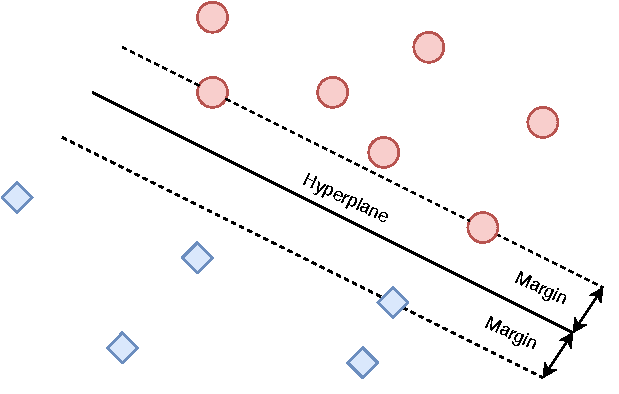
\includegraphics[scale=1]{svm}
\centering
\caption{A hyperplane that separates examples of negative and positive classes with maximal margin}
\label{fig:svm}
\end{figure}
Support vector machines (SVM) are supervised machine learning algorithms that are used for classification and regression analysis.
A single SVM algorithm separates data to two classes by defining a hyperplane that has a maximal distance (margin) to examples of opposing classes (Figure \ref{fig:svm}).
The hyperplane is defined with labeled training data and prediction happens by defining the side in which the example is placed in. If a hyperplane which cuts the data perfectly so that each example is on it's own side is not possible, the algorithm tries to find a division so that as few an example are on the wrong side as possible \cite{hotho}.

In the case that the given classes can not be separated linearly, SVM transforms ("maps") the input space into a higher dimensional space in which regions can be linearly separated \cite{rigutini2004}.
Support vector machines can also be used for unsupervised learning, when there is no labeled data, to find a natural grouping by using Support Vector Clustering (SVC) \cite{ben-hur2001}.

SVMs have shown good results in text categorization in the past, are quite computationally efficient and generalize well.
Another strength of SVM is that it rarely requires feature selection given that it inherently picks support vectors (individual datapoints) needed for good classification \cite{hotho}.

\subsection{Decision Trees} \label{Decision Trees}

\begin{figure}[t]
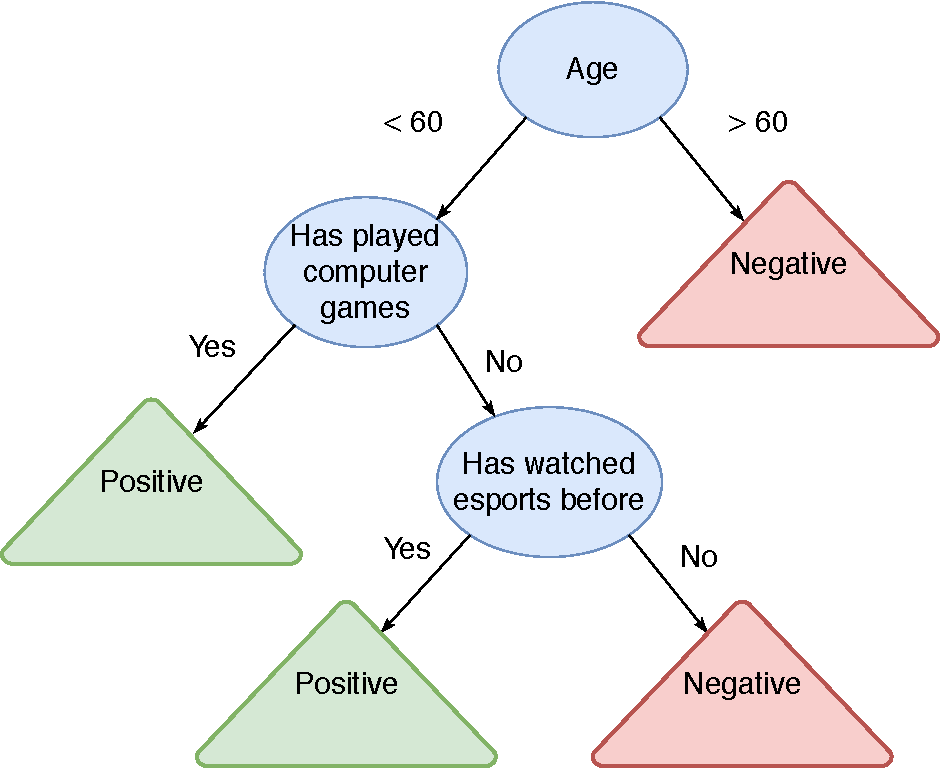
\includegraphics[scale=0.5]{decision_tree}
\centering
\caption{Example of a simple decision tree which predicts the sentiment of a person regarding esports}
\label{fig:decision_tree}
\end{figure}
Decision trees are classifiers that apply a set of rules sequentially to reach a decision.
They can be used for both regression and classification problems and have been among the most popular approaches used for text classification in the past \cite{hotho} \cite{rokach2005}.

Figure \ref{fig:decision_tree} depicts a simple decision tree with three round internal nodes and four triangular leaves.
Nodes are labeled with the testable attribute and branches with the attribute's values.

The training process of a text classification decision tree is as follows: Given a training set $M$ with labelled documents, find the word $t_i$ that best predicts the class of the documents.
Partition the training set into two subsets, $M^+_i$ and $M^-_i$, with $M^+_i$ containing examples with $t_i$ and $M^-_i$ containing examples without $t_i$.
Apply this procedure recursively to $M^+_i$ and $M^-_i$ until all the documents in a subset belong to the same class $L_c$.
The generated tree of rules has an assignment to a class as its leaves \cite{hotho}.

As can be seen from figure \ref{fig:decision_tree}, individual decision trees are quite simple to understand and to interpret, but are usually not competitive with other supervised learning approaches.
They can, however, be dramatically improved by combining multiple trees together to get a consensus prediction with approaches such as \textit{bagging, boosting and random forests} with the cost of losing some interpretability \cite{james2013}.

\subsection{Artificial neural network} \label{Artificial neural network}
\begin{figure}[t]
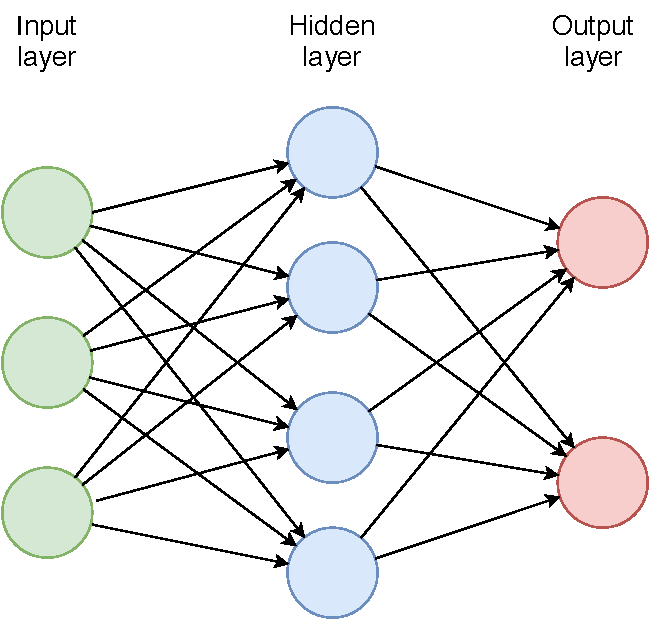
\includegraphics[scale=0.6]{nn}
\centering
\caption{Example of a simple feedforward neural network}
\label{fig:nn}
\end{figure}

A neural network consists of layers of simple processing elements called neurons that are connected to each other.
Each connection has an associated weight that is applied to input.
The first layer is called the input layer after which comes any number of intermediate, or hidden, layers followed by a final output layer.
Neurons are not interconnected within a layer but are only connected to the neurons in adjacent layers.
In a text classifier neural network the prediction of the network can be determined from the values of the final layer's neurons.
For example, a classifier with three different possible classes would have three neurons in the output layer, each corresponding to the probability of a single class \cite{pal1992}.

Neural networks are usually trained using backpropagation which finetunes the parameters of the network by first feeding the network training data, checking the output and if it is misclassified, and then backtracking and updating the weights of the network to eliminate or minimize the error \cite{sebastiani2002}.

The simplest neural network is the single-layer perceptron, introduced by Rosenblatt in 1958 \cite{rosenblatt1958}, which consists of a single hidden layer between an input layer and an output layer.

Since neural networks consist of simple building blocks, layers of neurons or other functions, stacked on top of each other, it allows designing of deep, complex architectures with practically infinite ways of combination.
The depth of a neural network is defined by the number of it's hidden layers.
The latest state-of-the-art neural network models consist of very deep networks with millions of parameters.

\section{Evaluation} \label{Evaluation}
Evaluating the performance of a classifier is an important step in order to define if the trained classifier actually learned something.

\textbf{True positive, true negative, false positive and false negative} (TP, TN, FP, FN, respectively), are labels used to define the classification result of a single example in a classification task.
If the classifier correctly predicts that the example is positive (e.g. a piece of text belongs to class 1), the example is considered a true positive.
In the case when a negative example is correctly predicted, it is a true negative.
If the classifier wrongly predicts that the example is positive when it is actually negative, or vice versa, the result is a false positive of a false negative.
Depending on the case, a classifier can have requirements such as to minimize the false negative or false positive rate.

Figure \ref{fig:confusionmatrix} depicts a \textbf{confusion matrix} which is a common way to visualize classification results.

\begin{figure}[t]
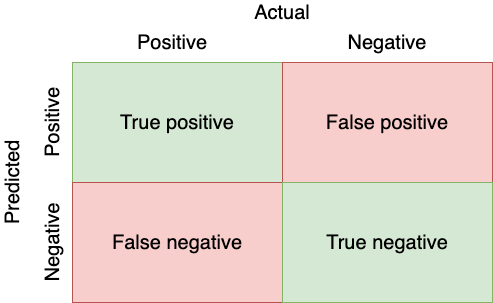
\includegraphics[scale=0.6]{confusionmatrix}
\centering
\caption{A confusion matrix.}
\label{fig:confusionmatrix}
\end{figure}

The simplest metric to use is \textbf{accuracy} (equation \ref{accuracy}), which defines the fraction of correctly classified documents (true positives and true negatives) in relation to the total number of documents.
It is a raw metric that doesn't give a whole lot of insight into the performance of the classifier in such cases where the training data is not evenly distributed.
\begin{equation}\label{accuracy}
  \dfrac{TP + TN}{TP+TN+FP+FN}
\end{equation}

\textbf{Precision} (equation \ref{precision}) defines the accuracy for positive example predictions, e.g. how many of the texts that we classified as 1 were actually 1.
It only takes into account positive predictions that were either true or false.
\begin{equation}\label{precision}
  \dfrac{TP}{TP+FP}
\end{equation}

\textbf{Recall} (equation \ref{recall}) defines the proportion of positive examples actually predicted as positive, e.g. how many of the positive examples did the classifier get right.
\begin{equation}\label{recall}
  \dfrac{TP}{TP+FN}
\end{equation}

\textbf{Specificity} (equation \ref{specificity}) defines the proportion of negative examples that were correctly predicted as negative, e.g. how many of the negative examples did the classifier get right.
Specificity is the opposite of recall.
\begin{equation}\label{specificity}
  \dfrac{TN}{TN+FP}
\end{equation}

\textbf{F-score} or $F_1$ score (equation \ref{fscore}) combines recall and precision in an effort to capture their properties in a single value.
It is the harmonic mean of precision and recall.

\begin{equation}\label{fscore}
  F=\dfrac{2}{1/recall + 1/precision}
\end{equation}

F-score is a commonly used metric to describe system performance in machine learning but it is criticized for lacking detail \cite{derczynski2016}.
Two different models that have the same F-score on the same task are not necessarily successful in the same way.

\textbf{Complementarity} \cite{brill1998} is a measure of the difference in decisions made by two classifiers which attempts to capture the properties that F-score misses.
It represents the amount of times when the other classifier was correct and the other wasn't \cite{derczynski2016}.

Clearly, choosing a single metric to represent the performance of a classifier seems naive.
Thus, in order to gain insight into actual performance one has to calculate a number of metrics.

\chapter{Deep learning in natural language processing} \label{Deep learning in natural language processing}
Deep learning is a branch of machine learning and a re-branded name for neural networks.
All of machine learning can be defined as learning to predict the future based on past observations.
In addition to learning to predict, deep learning also tries to represent the data in such a form that it is suitable for prediction.
Given a large amount of desired input-output mappings, deep learning feeds the data into a network that successively transforms the data until a final transformation predicts the output.
The transformations are learned from the mappings such that each successive transformation makes it easier to relate the data to the given label.
After a human designer defines the architecture and training regime of the network, gathers and preprocesses a proper set of input-output examples and encodes the data, the network can automatically learn how to best produce this mapping \cite{goldberg2017}.

This chapter gives an overview of transfer learning in section \ref{Transfer learning}, delves deeper into how a deep learning model is trained in section \ref{Training}, provides an overview of different relevant architectures in section \ref{Architectures} and finally describes the methodology of three modern machine learning models: ULMFit, BERT and ELECTRA, in section \ref{Modern models}.

\section{Transfer learning} \label{Transfer learning}
Transfer learning refers to the ability of a system to reuse knowledge learned in a previous task in a task of new or novel domain that shares some commonality with the previous task \cite{yang2020}.
Often the motivation for using transfer learning comes from a lack of labelled training data for a specific task.
In natural language processing it is widely used to first train a model on a general domain corpus of fully or partly unlabelled data, so that it learns the generalities of the given language (a \textit{language model}), and then fine-tuning the model on some downstream task, such as classification.

All of the introduced NLP-models later in this chapter use transfer learning as each has a clear distinction between the pre-training and fine-tuning phases in model training where another model's pre-trained state can be transferred to another task and fine-tuned further for that task.

\subsection{Language modeling}\label{Language modeling}
Language modeling is the task of assigning a probability to sentences in a language.
In addition to assigning a probability to sequences of words, language models also define the probability that a word follows a sequence of words.
Language modeling is an important part in several real-world applications such as speech recognition and machine-translation, where language models are used to score the transcriptions and translations that the systems output.

The formal definition of language modeling is to assign a probability to any sequence of words $P(w_{1:n})$, which can be rewritten as:

\begin{equation}
  P(w_{1:n})=P(w_1)P(w_2|w_1)P(w_3|w_{1:2})P(w_4|w_{1:3})\ldots{}P(w_n|w_{1:n-1}).
\end{equation}

using the chain-rule of probability.
What this means is that the probability of a sequence of words is defined by the probabilities of each word $n$ following the previous $n-1$ words.
In the past, language models made use of the \textit{markov-assumption} that states that the future is independent of the past given the present.
Nowadays, with modern architectures such as recursive neural networks, this assumption can be abandoned and models can condition on entire sentences while taking word order into account, which has lead to impressive gains in language modeling \cite{goldberg2017}.

Modern NLP networks are often pre-trained as language models before they are fine-tuned for a specific task.
Pre-trained language models can thus be used as a starting point for a model, transferring knowledge from a previous task.

\subsection{Embeddings} \label{Embeddings}
A common use case of transfer learning in NLP has been to use word embeddings that encode some information about a word in relation to other words in the feature space.
Using embeddings is a general way of transferring knowledge as it doesn't depend on any specific model architecture but only on the language used.
The most popular methods for generating vector representations for words have been Word2Vec \cite{mikolov2013}, GLoVe \cite{pennington2014}, and fastText \cite{bojanowski2017}.
% All of these methods can be seen as relying on the 'distributional hypothesis' as a heuristic applied for learning semantic similarities between words \cite{harris1954}.
The following subsections give an overview on these methods.

\subsubsection{Word2Vec} \label{Word2Vec}
Word2Vec is an open-source project based on the work by Mikolov et al. that can be used to train distributed representations of words and phrases \cite{mikolov2013}.

\begin{figure}[t]
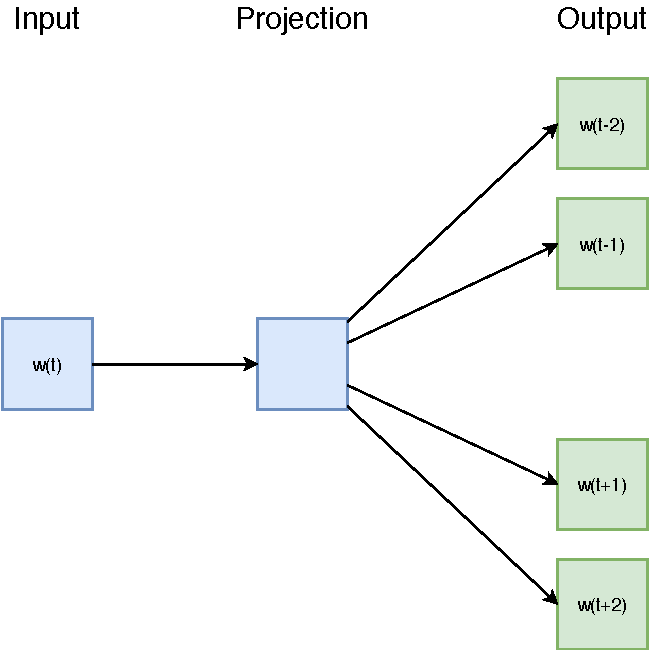
\includegraphics[scale=0.8]{skipgram}
\centering
\caption{Skip-gram model architecture.}
\label{fig:skipgram}
\end{figure}

It uses a skip-gram model (figure \ref{fig:skipgram}), proposed by Mikolov et al. in an earlier work \cite{mikolov2013a}, which is a prediction-based method.
The training objective of the skip-gram model is to find useful word representations for predicting the surrounding words in a sentence or a document.
It learns these representation by predicting the surrounding words for each word in a sentence within a defined max distance from the word.
Mikolov et al. show, that the produced representations exhibit linear structure that makes precise analogical reasoning possible \cite{mikolov2013}.

Given the computationally efficient model architecture of the skip-gram, the training times of Word2Vec are manageable even with huge amounts of data.

\subsubsection{GLoVe} \label{GLoVe}
Global Vectors for Word Representation (GLoVe) is a model to construct word representations.
It is a global log-bilinear regression model that combines the advantages from both Word2Vec-style local context window methods and global matrix factorization.
Training of GLoVe is done on aggregated global word-word co-occurrence statistics \cite{pennington2014}.

Given the same corpus and equal compute, Pennington et al. show that it outperforms Word2Vec and achieves better results faster \cite{pennington2014}, although Levy et al. \cite{levy2015} came to the opposite conclusion after careful testing.

\subsubsection{fastText} \label{fastText}
fastText is an open-source library for learning word embeddings and text classification.
It builds on the work of Word2Vec and improves on the skip-gram model by incorporating character n-grams in it.
Words are now represented as a sum of n-gram vectors instead of a single vector.
This is especially important for morphologically rich languages, such as Finnish, that contain many word forms that occur rarely in the training corpus, which makes learning good word representations difficult \cite{bojanowski2017}.

Mikolov et al. show that fastText significantly outperforms GLoVe on a number of tasks \cite{mikolov2017}.


\section{Training} \label{Training}
The goal of a neural network is to return a function $f()$ that accurately maps input examples to their labels.
To make it more precise, a \textit{loss function} is introduced to quantify the loss suffered when predicting examples in the training set.
A loss function assigns a numerical score to predicted outputs given the expected, true outputs.
The function is bounded from below such that the minimum value is only attainable in cases where the prediction is correct.
The goal of the training algorithm is then to minimize the average loss over all training examples \cite{goldberg2017}.

Attempting to minimize the loss at all costs may result in \textit{overfitting} the training data, thus a soft restriction on the loss function is applied in the form of a \textit{regularization term}, which tracks the ``complexity'' of parameters.
Thus the objective of the optimization problem becomes keeping a balance between low loss and low complexity \cite{goldberg2017}.

\subsection{Loss functions}\label{Loss functions}
\subsubsection{Binary cross entropy loss}\label{Binary cross entropy loss}
Binary cross entropy loss, also referred to as \textit{logistic loss} is a loss function used in binary classification with conditional probability outputs.
A set of two target classes labeled 0 and 1 is assumed, with a correct label $y\in{}\{0,1\}$.
The output of the classifier, $\tilde{y}$, is transformed to the range $[0, 1]$ using the sigmoid function $\sigma{}(x)=1/(1+e^{-x})$, and is interpreted as the conditional probability $\hat{y}=\sigma{}(\tilde{y}) = P(y=1|x)$.
The rule for prediction is:
\begin{equation}
prediction =
\begin{cases}
  \  0,\ \ \hat{y}\ <\ 0.5\\
  \ 1,\ \ \hat{y}\ \geq \ 0.5\\
\end{cases}
\end{equation}

The network maximizes the log conditional probability $\log\ P(y = 1|x)$ for each training example $(x,y)$.
Logistic loss is defined as:
\begin{equation}
  L_{logistic}\ (\hat{y},y)=-y\log\ \hat{y}-(1-y)\log\ (1-\hat{y}).
\end{equation}

The logistic loss is useful when we want the network to produce class conditional probability for a binary classification problem.
It is assumed that the output layer is transformed using the sigmoid function when using the logistic loss \cite{goldberg2017}.

\subsubsection{Categorical cross-entropy loss}\label{Categorical cross-entropy loss}
The categorical cross-entropy loss is a loss function that is used when a probabilistic interpretation of the scores is desired.
Let $y=y_{[1]},\ldots{},y_{[n]}$ be a vector representing the true multinomial distribution over the labels $1,\ldots{},n$, and let  $\hat{y}=\hat{y}_{[1]},\ldots{},\hat{y}_{[n]}$ be the linear classifier’s output transformed by the \textit{softmax} function, and represent the class membership conditional distribution $\hat{y}_{[i]} = P(y=i|x)$.
The softmax function forces the values of the output to be positive and sum to 1, thus making the output interpretable as a probability distribution.

The categorical cross entropy loss measures the dissimilarity between the true label distribution $y$ and the predicted label distribution $\hat{y}$, and is defined as cross entropy:
\begin{equation}
  L_{cross-entropy}\ (\hat{y},y)=-\sum_{i}y_{[i]}\log (\hat{y}_{[i]}).
\end{equation}

The case when each training example has only a single correct class assignment is called hard classification.
In such cases y is a one-hot vector representing the true class, and the cross entropy can be simplified to:
\begin{equation}
  L_{cross-entropy(hard classification)}\ (\hat{y},y)=-\log(\hat{y}_{[t]}),
\end{equation}
where $t$ is the correct class assignment.
This equation attempts to set the probability mass assigned to the correct class $t$ to 1.
Increasing the mass assigned to the correct class means decreasing the mass assigned to all the other classes given that the scores $\hat{y}$ have been transformed using the softmax function to be non-negative and sum to one.

The cross-entropy loss is widely used in log-linear models and neural networks.
It produces a multi-class classifier which predicts a distribution over all possible labels in addition to predicting the best class label.
When using the cross-entropy loss, it is assumed that the classifier’s output is transformed using the softmax function \cite{goldberg2017}.



\subsubsection{Ranking losses}\label{Ranking losses}
Margin-based ranking loss can be used in cases where supervision is not given as labels but as pairs of correct and incorrect samples $x$ and $x'$, and where the goal is to give a higher score to correct items.
Such a situations may occur when the training set consists of only positive examples and the generation of negative examples is done by corrupting positive ones.
Margin-based ranking loss is defined as follows for a pair of correct and incorrect samples:
\begin{equation}
  L_{ranking(margin)}(x,x')=\max(0, 1 - (f(x) - f(x'))),
\end{equation}
where $f(x)$ is the score assigned by the classifier for input vector $x$.
The objective of the function is to rank correct inputs above incorrect ones with a margin of at least 1.

Ranking loss is used in language tasks such as deriving pre-trained word embeddings (section \ref{Embeddings}) given a correct and corrupted word sequence, and the goal being to rank the correct sentence over the corrupt one \cite{goldberg2017}.


\subsection{Stochastic Gradient Descent}

Stochastic gradient descent (SGD) is a general optimization algorithm which powers nearly everything in deep learning.
The goal of the algorithm is to minimize the total loss over the training set by repeatedly sampling a training example and computing the gradient of the error on the example \cite{goldberg2017}.

Sampling each individual example and calculating a gradient for them quickly becomes infeasible when training set sizes are large, thus SGD uses \textbf{minibatching} to draw a uniform set of examples at a time from the training set to compute a gradient for.
The gradient is then propagated though the network and a new gradient is calculated from the next minibatch \cite{goodfellow2016}.

\textit{Learning rate} is a parameter that defines the amount that the weights of the network are updated with each gradient.
It is a small positive value, usually in the range $[0, 1]$.

Gradient descent has been regarded as slow or unreliable in the past.
Nowadays we know that it works great with neural networks even though it is not guaranteed that the algorithm will arrive even at a local minimum in a reasonable amount of time.
It however finds a very low value for the cost function quickly enough \cite{goodfellow2016}.

In addition to SGD, there exists other optimization algorithms which are used nowadays such as Adam \cite{kingma2017}, which is designed to define the learning rate on a minibatch basis.
Algorithms such as SGD+momentum \cite{polyak1964} are variants of SGD where the accumulated previous gradients affect the current update.

\section{Architectures} \label{Architectures}
\subsection{Recurrent Neural Network} \label{Recurrent Neural Network}

\begin{figure}[t]
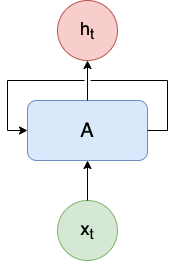
\includegraphics[scale=1]{rnnloop}
\centering
\caption{An RNN-module which illustrates the recurrent nature of the model}
\label{fig:rnnloop}
\end{figure}

Recurrent Neural Networks (RNN) are networks that process an input sequence one token at a time and maintain a state in its hidden units that contains information about the past elements in the sequence.
This approach has been proven to work well with tasks that contain sequential input such as speech, language and music \cite{lecun2015}.
Figure \ref{fig:rnnloop} shows the basic methodology behind an RNN: a chunk of neural network, A, looks at the input $x_t$ and outputs a value $h_t$. The output value is looped back as a second input value which allows for information to be passed from one step to the other.

\begin{figure}[t]
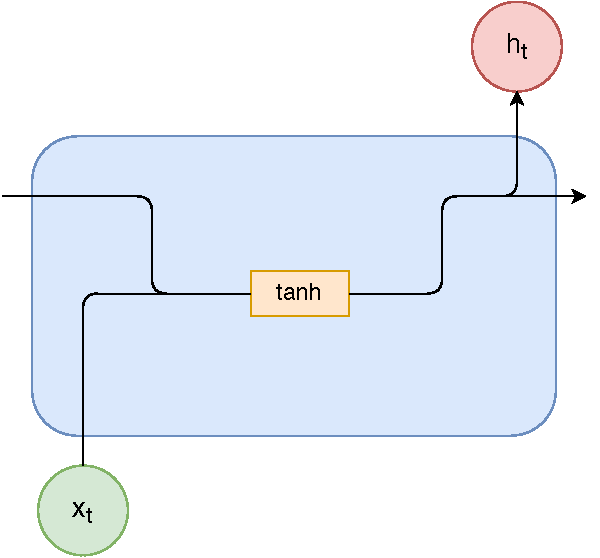
\includegraphics[scale=0.9]{rnn}
\centering
\caption{The insides of an RNN}
\label{fig:rnn}
\end{figure}

Figure \ref{fig:rnn} shows a visualization of the insides of an RNN module which is quite simple in practice. $x_t$ represents an input at timestep $t$, $tanh$ is a function that returns the hyperbolic tangent of the input and $h_t$ is the hidden state of the network at timestep $t$.
First the hidden state from the previous timestep and the current input value are added to each other after which the sum is fed into the $tanh$ function.
$tanh$ essentially squishes the input value between -1 and 1 to keep the values from exploding due to repeated multiplication.
The output of tanh is the new hidden state, the memory of the network, which is then fed to the next timestep.


The training of an RNN happens by using a variant of backpropagation called \textit{backpropagation through time} (bptt) which is a generalization of backpropagation for networks which store the activations of units while going forward in time \cite{rumelhart1985}.
The backward gradient update pass is thus also backward in time and recursively computes the required gradients with the saved activations.
It is easy to see how this works when the different timesteps of an RNN are unrolled and displayed as if they combine to make a single neural network with multiple layers (fig \ref{fig:rnn}).


RNNs have difficulties maintaining long-term dependencies when processing lengthy input sequences that originates from the \textit{vanishing gradients} problem \cite{bengio1994}:
During backpropagation gradients, with which the weights of the network are updated, change as they are applied backwards through time.
A small change to a layer before means an even smaller change in the current layer.
On the contrary, gradients with big changes tend to ``blow up''.
This means that the earlier layers in the network either stop learning since they only receive small gradient updates or their weights oscillate due to big changes \cite{hochreiter1997}.
In an RNN this problem is magnified due to backpropagation being applied to each time step.

\subsection{LSTM} \label{LSTM}
Long short-term memory (LSTM) is a recurrent network architecture proposed by Hochreiter and Schmidhuber in 1997 \cite{hochreiter1997}.
LSTM was designed to combat the vanishing gradients problem that is especially prevalent in RNNs.
LSTMs work exceptionally well on a large variety of problems and are widely used nowadays.

\begin{figure}[t]
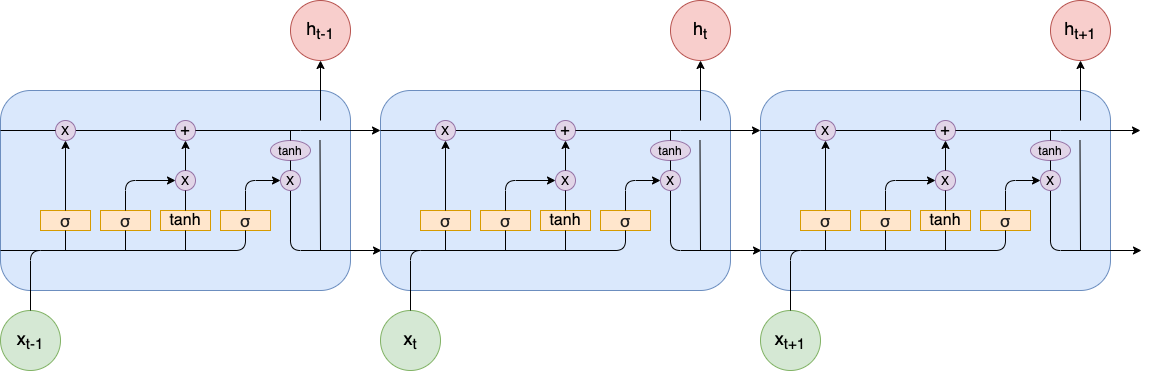
\includegraphics[scale=0.9]{lstm}
\centering
\caption{Long short-term memory network}
\label{fig:lstm}
\end{figure}

Figure \ref{fig:lstm} illustrates an lstm module. Each line carries a vector, merging lines denote concatenation, forking lines denote copying of the vector and each copy going to different directions, orange boxes are learned neural network layers and purple circles represent pointwise operations such as multiplication, addition and hyperbolic tangent.
In addition to keeping track of the hidden state of the network, LSTM adds another state called cell state that is denoted by the horizontal line running through the top of the figure.
Information is added and removed to the cell state by gates that are made up of sigmoid ($\sigma$) neural net layers and pointwise multiplication operations.
A sigmoid neural net layer takes as input the concatenation of the previous hidden state $h_{t-1}$ and the current input $x_t$ and output a vector of values between 0 and 1 to describe how much of each value is to be let through.
A value of 1 lets everything through while a 0 lets nothing through.
An LSTM has three of these gates.
From left to right, the first gate forms the forget gate layer which decides what data to keep and what to discard from the previous cell state.
Next, the data to add to the cell state is decided with a combination of a $sigmoid$ layer and a $tanh$ layer. The $tanh$ layer outputs new candidate values and the $sigmoid$ layer decides which of them to add to the cell state.
Finally, the last layer determines the output (hidden state) of the cell by taking the current cell state's values and applying a $tanh$ function to push the values between -1 and 1 and multiplying them with the output of the $sigmoid$ gate.
The new cell state and hidden state are then passed on to the next time step.

The LSTM architecture described above is considered a standard version of LSTM, but other variants exist too.
One popular variant of LSTM introduced by Gers \& Schmidhuber \cite{gers2000a} adds peephole-connections that allow the gate layers to look at the cell state.
Another variant called the \textbf{Gated Recurrent Unit} (GRU, figure \ref{fig:gru}), introduced by Cho, et al. \cite{cho2014}, simplifies the model by combining the forget and input gates into a single update gate.

\begin{figure}[t]
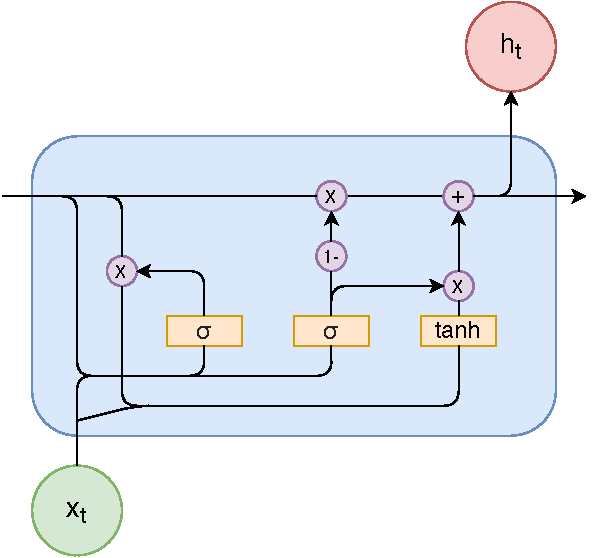
\includegraphics[scale=0.9]{gru}
\centering
\caption{Gated Recurrent Unit}
\label{fig:gru}
\end{figure}

\subsection{Transformer} \label{Transformer}
RNNs, as presented before, are inherently sequential in nature.
They take an input at timestep $t$ and compute a hidden state $h_t$ with knowledge from the previous hidden state $h_{t-1}$.
This sequentiality prohibits efficient parallelization within training examples since one has to come before the other in training.
Parallelization across examples is also critically constrained by memory at longer sequence lengths.
In addition to this, RNNs suffer from the so-called \textit{vanishing gradient problem} which is exacerbated at longer sequence lengths \cite{vaswani2017}.

Attention is a mechanism that allows the modeling of dependencies without regard for distance in input or output sequences.
It has been used in conjunction with recurrent neural networks to achieve good results, but using it with RNNs somewhat limits the power of attention since the model is still constrained by the aforementioned problems of RNNs.
Thus Vaswani et al. proposed a novel architecture in 2017, the Transformer, to combat these limitations.
The Transformer has been the foundation of neural networks that have achieved state-of-the-art results in various language-related tasks in the last couple of years \cite{vaswani2017}.

The Transformer consists of an encoder, which maps an input sequence of tokens to a sequence of continuous representations, and a decoder, which takes a continuous representation and generates an output sequence.
The output sequence is generated one token at a time while taking the previous generated tokens as additional input.

\begin{figure}[t]
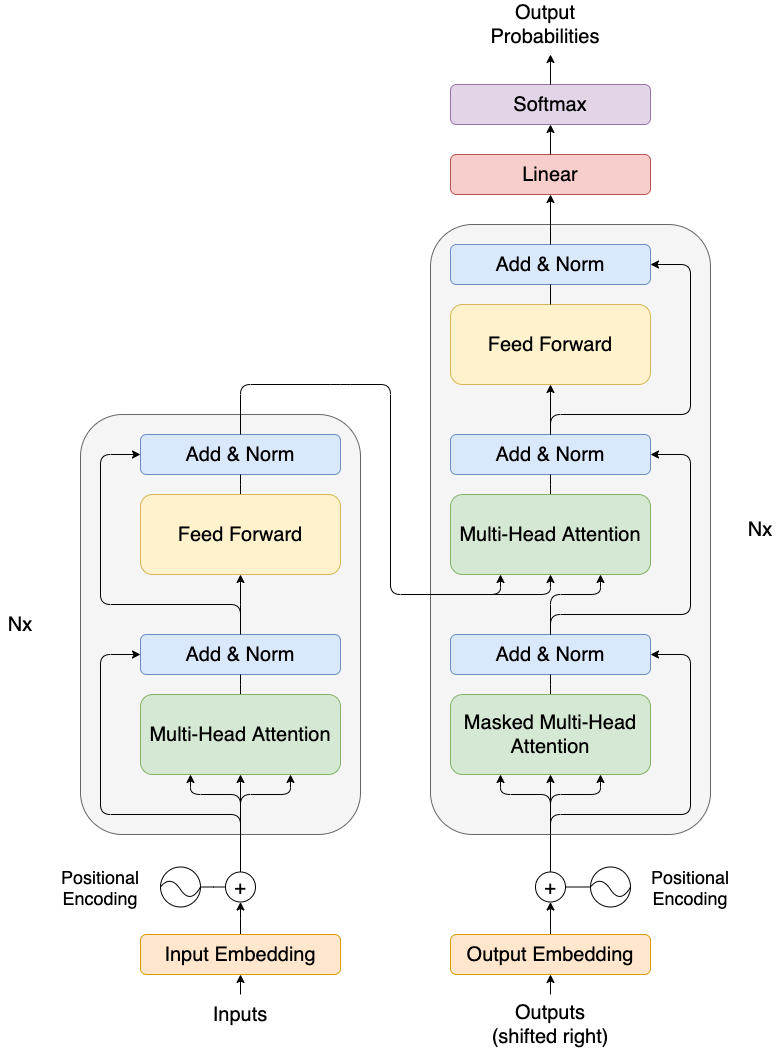
\includegraphics[scale=0.5]{transformer}
\centering
\caption{The Transformer, from Vaswani et al. 2017 \cite{vaswani2017}}
\label{fig:transformer}
\end{figure}

The overall architecture of the Transformer is shown in Figure \ref{fig:transformer}, with the left side of the figure representing the encoder and the right side the decoder.
The encoder is composed of six identical layers stacked on top of each other.
Each layer consists of two sub-layers; a multi-head self-attention mechanism and a fully connected feed-forward network.
Residual connections \cite{he2016} are used around each sub-layer to shortcut the sub-layers while training.
This leads to faster training times and a more robust model as the connections are gradually restored during training.
Finally, layer normalization is applied to the output of the sub-layer as $LayerNorm(x+Sublayer(x))$, where $Sublayer(x)$ refers to the function implemented by the sub-layer.
Due to the residual connections, all sub-layers and embedding layers have to produce outputs of the same dimensionality.
Thus in the Transformer the dimensionality is defined as $d_{model}=512$.

The decoder is also composed of six identical layers but additionally includes a third sub-layer, which applies multi-head attention over the output of the encoder stack.
The self-attention sub-layer in the decoder stack is also modified to prevent positions from attending to subsequent positions.
Thus predictions for position $i$ can only depend on the outputs before $i$.

Attention can be described as a function of mapping a query and a set of key-value pairs to an output.
The query, keys, values and output are all vectors.
The output is a weighted sum of the values, where the weight of each value is defined by a compatibility function of the query with the corresponding key.
The particular version of attention in the Transformer is called \textit{Scaled Dot-Product Attention} in which the input consists of queries and keys of dimension $d_k$ and values of dimension $d_v$.
The dot products of queries with all keys are computed first, denoted by $QK^T$ in equation \ref{eq:attention}.
The results are divided by $\sqrt{d_k}$ and then a softmax function is applied to obtain the weights on the values \cite{vaswani2017}.


\begin{equation}
  Attention(Q,K,V)=softmax(\dfrac{{QK^T}}{{\sqrt{d_k}}})V\label{eq:attention}
\end{equation}

Instead of using a single attention function over all the keys, values and queries with dimension $d_{model}$, the Transformer uses so-called \textit{Multi-Head Attention} to linearly project the keys, values and queries $h$ times to $d_k$, $d_k$ and $d_v$ dimensions.
The attention function is then applied in parallel to all these projected versions, yielding $d_v$-dimensional outputs.
These outputs are then concatenated and projected to achieve the final result.
This allows the model to jointly attend to information from different representation subspaces at different positions.
In the Transformer, 8 parallel attention heads are used \cite{vaswani2017}.

Attention is used in three different ways in the Transformer.
In encoder-decoder attention, where the output of the encoder is used in the decoder, the queries come from the previous decoder layer and the keys and values come from the output of the encoder, and in encoder and decoder self-attention.
In encoder self-attention all the queries, keys and values come from the output of the previous encoder layer, thus each position in the encoder can attend to all positions in the previous encoder layer.
Decoder self-attention similarly receives its input from the previous decoder layer's output, but doesn't allow attention over all the positions but only up to and including the current position.
This is achieved by masking out all the input values of the softmax corresponding to illegal connections.

The decision to use self-attention was made based on three requirements: to minimize the total computational complexity of each layer, to maximize the amount of parallelizable computation and to minimize the path length between long-range dependencies.
A side benefit of self-attention is more interpretable models as attention distributions can be inspected and tested with different examples to gain insight into the behaviour of individual attention heads \cite{vaswani2017}.

\subsection{Other architectures} \label{Other architectures}
\subsubsection{Autoencoder}\label{Autoencoder}
Autoencoders are neural networks that are trained to attempt to copy its input to its output.
They compress the input into a lower-dimensional representation after which they attempt to reconstruct the original input from this representation.
An autoencoder that succeeds at a perfect copy is not very useful, thus they are designed to be unable to learn to copy perfectly.
Because the model has to prioritize which aspects of the input should be copied, it often learns useful properties of the data \cite{goodfellow2016}.


\begin{figure}[t]
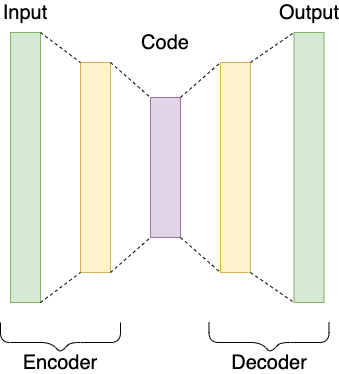
\includegraphics[scale=1]{autoencoder}
\centering
\caption{The autoencoder}
\label{fig:autoencoder}
\end{figure}

An autoencoder consists of three components: an encoder, code and a decoder.
The encoder compresses the input and produces the code, the decoder reconstructs the input from the code.
Figure \ref{fig:autoencoder} illustrates the simple architecture of the autoencoder.
Both the encoder and the decoder are fully connected feedforward networks and are essentially mirror images of each other.
The only requirement of the autoencoder is that the input and output dimensions are the same.

Autoencoders have traditionally been used for dimensionality reduction or feature learning \cite{goodfellow2016}.
For natural language processing, Variational Autoencoders \cite{kingma2014} have been used for generative document modelling and supervised question answering \cite{miao2016}.



\subsubsection{Convolutional Neural Network}\label{CNN}
\begin{figure}[t]
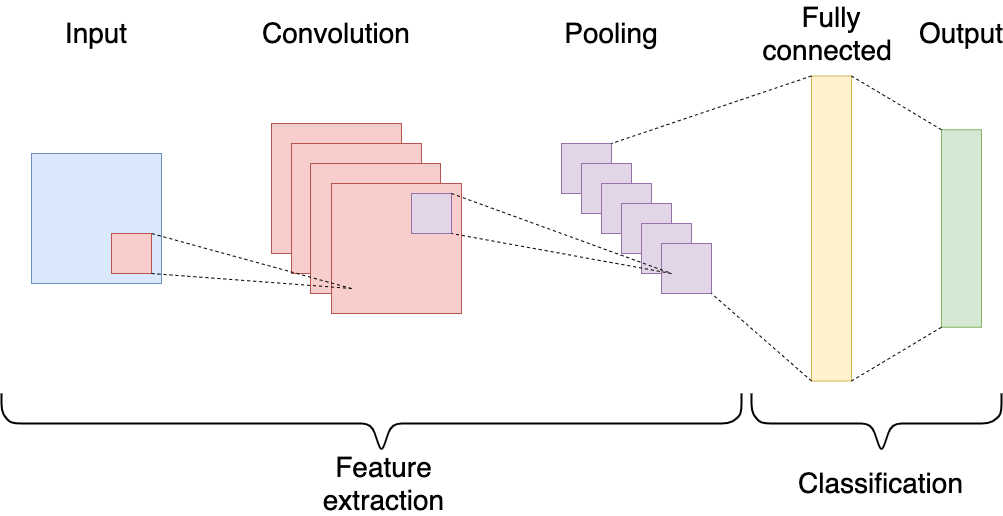
\includegraphics[scale=0.55]{cnn}
\centering
\caption{A convolutional neural network for classification}
\label{fig:cnn}
\end{figure}
Convolutional Neural Networks (CNN) are networks that incorporate convolutional and pooling layers into a neural network.
CNN's have four key ideas that take advantage of the properties of signals: shared weights, pooling, local connections and the use of many layers.
A typical CNN (Figure \ref{fig:cnn}) is structured as a series of stages.
The first stages are composed of convolutional layers and pooling layers.
Convolutional layers try to detect local conjunctions of features from the previous layer.
A convolutional layer's units are organized in feature maps, within which each unit is connected to local patches in feature maps of the previous layer.
These connections are weighted and the weights are contained in a filter bank, that is shared within all the units of a feature map.
Every feature map thus has it's own filter bank.
The role of the pooling layers is to merge semantically similar features into one.
They reduce the dimension of the representation in an effort to make the network more robust against small shifts and distortions in the data.
Stacks of convolutions and pooling are finally followed by fully-connected layers that are trained to output the result \cite{lecun2015}.


Convolutional neural networks have been used for a multitude of tasks in natural language processing in the past such as sentiment classification and sentence modeling \cite{kalchbrenner2014}.


\section{Modern models} \label{Modern models}

\subsection{ULMFiT} \label{ULMFiT}
Universal Language Model fine-tuning (ULMFiT) is a transfer learning based methodology for text classification which posted state-of-the-art results when it was published in 2018.
It consists of firstly pre-training a language model on a general-domain corpus and then fine-tuning it on a classification task.
This idea of first pre-training on a large general corpus and then fine-tuning it has been tried before, but has proven to be a challenging task due to it requiring millions of in-domain documents to achieve good performance \cite{dai2015}.
With ULMFiT Howard et al. proposed novel training techniques to make the training feasible even with a small corpus \cite{howard2018}.

ULMFiT is a \textit{universal} method in that it uses a single architecture and training process, requires no custom feature engineering, works across tasks with variable document sizes and label types, and doesn't require additional in-domain documents or labels \cite{howard2018}.

ULMFiT uses a 3-layer weight-dropped long shot-term memory (AWD-LSTM) network, proposed by Merity et al. \cite{merity2017}, which is a recurrent neural network (RNN).
AWD-LSTM is a vanilla LSTM with various regularization and optimization strategies such as DropConnect \cite{wan}, which prevents over-fitting by randomly dropping connections between the recurrent hidden to hidden weight matrices, and averaged gradient descent as its optimization algorithm.

The training begins with pre-training a general-domain language model with unlabeled text data to capture the general properties of language.
This initial training step is the most expensive in the whole method but only needs to be done once.

After the general language model is trained, it is fine-tuned with the target task data.
This fine-tuning converges faster than the initial pre-training since the model needs to only adapt to the idiosyncrasies of the fine-tuning data.
This allows the training of robust language models even with small datasets.
ULMFiT uses \textit{discriminative fine-tuning} and \textit{slanted triangular learning rates} for the fine-tuning step of the language model.
With discriminative fine-tuning, instead of using a single learning rate for all the layers in the model, each layer is fine-tuned with a learning rate of its own.
The motivation for this comes from the fact that different layers capture different types of information, thus each layer should be fine-tuned for different amounts.
With slanted triangular learning rates, the learning rate is first linearly increased in order to get the model to quickly converge to a suitable region, and then linearly decreased to refine its parameters.

For the final step, two additional linear blocks are added to the end of the network, and the final classifier is fine-tuned with \textit{gradual unfreezing}.
Gradual unfreezing is used to prevent \textit{catastrophic forgetting} by unfreezing the layers of the model one by one, starting from the last.
Unfrozen layers are fine-tuned for one epoch after which the next layer is unfrozen until all the layers of the model have been unfrozen.
The whole model is then fine-tuned until convergence \cite{howard2018}.

Although outshined by BERT and other huge transformer-based models, ULMFiT is much fast to train and typically does not require a lot of data to get good results.



\subsection{BERT} \label{BERT}
Bidirectional Encoder Representations from Transformers (BERT) is a language representation model based on the Transformer \cite{vaswani2017} architecture (subsection \ref{Transformer}).
It uses a \textit{fine-tuning} based approach, in which all the pre-trained parameters are fine-tuned when applying pre-trained language representations to down-stream tasks, as opposed to a \textit{feature-based} approach, where the pre-trained representations are only used as additional features in a task-specific architecture.

Both the fine-tuning and feature-based approach share the same objective function during pre-training of learning general language representations by using unidirectional language models.
BERT uses a \textit{masked language model} (MLM) pre-training objective to achieve bi-directionality in context, thus allowing the model to see both left and right of the input token when training.
MLM randomly masks tokens in the input, and the objective is to predict the vocabulary id of the masked token based on its context.
BERT also uses a \textit{next sentence prediction} (NSP) task that jointly pre-trains text-pair representations \cite{devlin2019}.

As with ULMFiT, BERT also has a unified architecture across different tasks with a minimal difference between the pre-trained architecture and the final downstream one.
BERT's architecture is almost identical with the Transformer described in section \ref{Transformer}, the difference comes mainly in the number of layers (Transformer blocks), denoted as $L$, hidden size, denoted as $H$ and the number of attention heads, denoted as $A$.
Results for BERT performance was primarily reported for two sizes: $BERT_{BASE}$ (L=12, H=768, A=12, total parameters=110M) and $BERT_{LARGE}$ (L=24, H=1024, A=16, total parameters=340M).

BERT uses WordPiece embeddings \cite{wu2016}, essentially similar to SentencePiece embeddings (section \ref{SentencePiece}).
Pre-training happens by the two aforementioned unsupervised tasks: Masked language modeling and next sentence prediction.

In MLM, 15\% of all WordPiece tokens are randomly chosen and each chosen token has an 80\% chance to actually be masked, a 10\% chance to be replaced with a random token, and a 10\% chance to stay unchanged.
The reason for not always masking the chosen tokens is because the [MASK] token does not appear during fine-tuning, causing a mismatch between the two steps otherwise.

In NSP, training examples consist of two sentences $A$ and $B$.
50\% of the time $B$ is actually the next sentence that follows $A$ (label $IsNext$) and 50\% of the time it is a random sentence from the corpus (label $NotNext$).

With the use of the Transformer-architecture, WordPiece embeddings and two pre-training objectives that allow bidirectional context, BERT was able to exceed the state-of-the-art on multiple downstream tasks \cite{devlin2019}.

\subsection{ELECTRA} \label{ELECTRA}
Efficiently Learning an Encoder that Classifies Token Replacements Accurately (ELECTRA) is a further elaboration on the BERT model by Clark, et al. \cite{clark2020}
The primary motivation for ELECTRA is making pre-training more efficient given that training a full-sized BERT or any derivation of it (ALBERT, RoBERTa etc.) requires a considerable amount of compute and training data.
As described in the BERT chapter (chapter \ref{BERT}), BERT uses masked language modeling as a pre-training objective.
This MLM is inherently quite inefficient in its usage of the training data; only the masked tokens, approximately 15\% of the data, needs to be predicted.
As an alternative, ELECTRA proposes \textit{replaces token detection}, a pre-training task in which the model has to predict whether or not a token is the original token in the corpus or if it has been swapped for a token generated by a small masked language model.
This also solves the mismatch in BERT where the model sees [MASK] tokens during pre-training but not during fine-tuning.
ELECTRA trains the network as a discriminator rather than a generator, since it is predicting whether an input is corrupted or not.
This way ELECTRA learns from all the input tokens, rather than a small subset of them.

ELECTRA substantially outperforms MLM-based methods given the same amount of data and compute and works well even with relatively small amounts of compute \cite{clark2020}.

\chapter{Medical report document classification} \label{Medical report document classification}

\section{Problem definition} \label{Problem definition}

Doctors diagnose multiple patients each day from which a medical report is written and stored in a database.
The report usually consists of a written statement regarding the patient and the visit, and an according diagnosis code.
As doctors are overworked and short on time, this step is usually done in a hurry which increases the chance of human error in both the written text and assigned diagnosis code.
Thus, automatically defining a proper diagnosis code based on the written text would reduce the chance of making an error and save some time on the doctors part.
Additionally, such methods could be used to analyze past data in order to validate the correctness of already given diagnosis labels.


To find out if it would be possible to automatically define the diagnosis of texts to a high enough certainty, a couple of deep learning -based models were trained on a binary classification task where the model was to predict whether a given text should have a certain knee-related diagnosis code or not.
Since compute resources were a major constraint, only approaches with a reasonable single-gpu training time were considered.
Thus, a pretrained and finetuned ULMFiT and ELECTRA, and a finetuned FinBERT (pretrained by Virtanen et al.~\cite{virtanen2019}), were chosen for comparison.
In addition to comparing the different models with each other, each model --- excluding FinBERT, which provided a vocabulary of it's own from pretraining --- was trained multiple times with different sizes of a vocabulary which was extracted from the medical texts to see if vocabulary size meaningfully impacted the results.
Given the success of BERT and it's WordPiece tokenization in various NLP tasks, SentencePiece was chosen as a tokenizer for ULMFiT as well.

\section{Data} \label{Data}
\subsection{Medical reports}\label{Medical reports}
The medical data for the work was provided by Auria services at the Turku university hospital.
It consists of doctor's statements with corresponding diagnosis codes and other metadata, such as date of visit and hospital ward, of patients in the Turku-region.
No metadata was utilized in the training data, only the written text and the corresponding diagnosis code.
Since the actual diagnosis code for the text appeared often in it, all diagnosis codes in text were masked with a [CODE] token in the training data to prevent the model from learning from them.
HTML-tags such as <br> were removed in preprocessing and texts that were deemed too short (less than 80 characters) were also removed from the training set.

After extracting the documents that had one of two knee-related diagnosis codes as positive samples, the class balance for the dataset was 85\% negative and 15\% positive samples.
The dataset was eventually balanced by upsampling the positive samples.
Overall, the data consisted of 175000 documents with varying lengths.
Token amounts were dependent on the size of the vocabulary used.

\subsection{General Finnish}\label{General Finnish}
Since receiving access to the actual medical data took some time and due to the fact that it was not allowed to be taken out of the hospital, the chosen models and code were additionally trained and tested on a general Finnish corpus that Virtanen et al. compiled for FinBERT \cite{virtanen2019}.
It is composed from three different sources: news articles, online discussions, and documents crawled from the Finnish internet, and consists of 3.3 billion tokens from 234 million sentences.
The total size of the corpus is roughly 30 times the size of the Finnish Wikipedia.
The corpus was extensively preprocessed by filtering out documents that had too high a ratio of digits, uppercase or non-Finnish alphabetic characters, or low average sentence length.
Additionally, documents that featured 25\% or more duplication were removed as well as heuristically defined undesirables~\cite{virtanen2019}.


\section{Compute resources} \label{Compute resources}
Compute resources for the project were provided by Auria services for the medical models, and CSC for the general Finnish models.

\subsection{CSC} \label{CSC}
CSC (IT Center for Science Ltd.) is a non-profit state enterprise owned by the Finnish state and higher education institutions in Finland.
It offers compute resources for scientific purposes to universities and upkeeps the FUNET network, which is the Finnish national research and education network.
CSC operates two supercomputers, namely Taito and Puhti, and is working on a new supercomputer, Mahti, that is scheduled to open for use some time in 2020.
For this project, Puhti was chosen since it provides an ``artificial intelligence partition'' with access to GPU nodes with multiple Nvidia V100 graphics cards.

\subsubsection{Puhti}\label{Puhti}
Puhti was launched on September 2, 2019.
It is an Atos cluster system and has a variety of different node types.

Puhti has 682 CPU nodes, with a theoretical peak performance of 1,8 petaflops, and an AI partition of 80 GPU nodes with a peak performance of 2,7 petaflops.
Each node is equipped with two Intel Xeon processors, code name Cascade Lake, with 20 cores each running at 2,1 GHz.
Each GPU node also has four Nvidia Volta V100 GPUs with 32 GB of memory each.
The nodes are equipped with 384 GB of main memory and 3,6 TB of fast local storage.
The AI partition is engineered to allow GPU-intensive workloads to scale well across multiple nodes~\cite{zotero-178}.

When working with Puhti on this project, the workflow consisted of coding and testing the neural networks locally first, and then using Slurm to run batch jobs on Puhti.
This lead to some additional overhead in time for the project since working simultaneously on two environments proved quite arduous.
Additionally, keeping tabs on the versions of code was very important since it could be altered in both locations, thus git \cite{zotero-186} was used for this version control.

\subsubsection{Slurm}\label{Slurm}
Puhti uses the Slurm workload manager \cite{zotero-174} to handle scheduling jobs for compute clusters.
It is an open-source, fault-tolerant, and highly scalable cluster management and job scheduling system for Linux clusters.
First, it manages the allocation of exclusive and/or non-exclusive access to compute nodes to users for some duration of time during which they can perform work.
Second, it provides a framework for starting, executing, and monitoring work on the set of allocated nodes.
Finally, it manages a queue of pending work to arbitrate the contention for resources~\cite{zotero-176}.


\subsection{Turku University Hospital} \label{Turku University Hospital}
For training models on the clinical data, access was granted to \textbf{Blackbird}, a computer for artificial intelligence owned by Auria services, with four Nvidia V100 graphics cards allowing simultaneous training of multiple models.
All training and handling of clinical data happened on this computer which is located in the hospital and behind the hospital firewall in order to ensure that the sensitive data and resulting models did not accidentally or otherwise leak into the outer world.


Although the architecture could have managed training a medium-sized BERT, it was considered too long of a task to reserve the compute resources for.
Additionally, there wasn't enough domain-specific data for such a task.


The workflow on Blackbird consisted of connecting to the linux-based computer using secure shell (SSH), using screen~\cite{zotero-180} to multiplex the connection to multiple shells, and running a training process on each shell.
Jupyter notebooks~\cite{zotero-182} were also used on the machine for data visualization and prototyping, and were accessed locally by using ssh tunneling~\cite{zotero-184}.

\section{Methods}\label{Methods}
\subsubsection{ULMFiT}\label{ULMFiT}
The fastai v1 -library was used for implementing ULMFiT\footnote{https://github.com/fastai/fastai}.
As the library's support for SentencePiece\footnote{https://github.com/google/sentencepiece} was at the time quite limited, a considerable amount of custom code had to be written to incorporate the sub-word tokenizer in the training process.
The scripts used for training ULMFiT with SentencePiece are open-sourced and can be found from\footnote{https://github.com/invisiblesheep/ulmfit-sentencepiece}.

\subsubsection{ELECTRA}\label{ELECTRA}
For training ELECTRA, the pretraining and finetuning scripts were used from the official github repository\footnote{https://github.com/google-research/electra}.
The code was forked in order to make some changes to it regarding finetuning and evaluation parameters\footnote{https://github.com/invisiblesheep/electra}.

\subsubsection{BERT}\label{BERT}
For finetuning FinBERT, HuggingFace's transformers library was ultimately used \cite{wolf2020}.
It provides pretraining and finetuning scripts for a multitude of transformer-based models, such as BERT, XLNet and RoBERTa.
% The code for finetuning FinBERT was taken from the official BERT github repository\footnote{https://github.com/google-research/bert}, and FinBERT itself can be found from\footnote{https://github.com/TurkuNLP/FinBERT}.

\subsubsection{Baseline models}\label{Baseline models}
\textbf{fastText}\footnote{https://github.com/facebookresearch/fastText} was trained as a baseline model.
In addition to providing word embeddings, fastText can be used as a classifier as well.
fastText obtains document vectors by averaging word embeddings after which it uses multinomial logistic regression for classification.
As with most neural network classifiers, a probability distribution over classes is gained as a result after applying the softmax function to the results.
It uses a bunch of tricks, such as hierarchical softmax, to up the speed of training the model.
Thus it's an order of magnitude faster to train than a deep learning model but it still is somewhat competitive with one.

In addition to fastText, the results of a random classifier averaged over four runs and a majority predictor, which always predicts negative in this case, are also reported as a baseline.

\section{Results}\label{Results}
A binary classifier was built to identify texts that had one of two knee-related diagnosis codes from the training data.
The data was divided into training, validation and test sets with a 80--10--10 split, and stratified so that each set had an equal percentage wise representation of the classes.

\begin{table}[t]
\begin{center}
\begin{tabular}{lcccc}
         & Accuracy & Precision & Recall & F1 \\
        \hline
FinBERT &   91.68 &   68.02   &    74.16 &  70.96   \\
ELECTRA-30K    &  90.40 &   66.06 & 73.72 & 69.68 \\
ELECTRA-50K  &   91.23 &   69.29 & 76.19 & 72.58 \\
ELECTRA-100K  &  91.46 &   69.64 & 76.14 & 72.74 \\
ULMFiT-30K  &  93.85 &  84.28 & 72.54 & 77.97 \\
ULMFiT-50K  & 93.98 &  82.91 & 75.41 & 78.98 \\
ULMFiT-100K  & 94.11 & 83.95 & 75.17 & \textbf{79.32} \\
fastText &  93.49 & 84.34 & 70.07 & 76.54 \\
Random &  50.02 & 15.01 & 50.19 & 23.11 \\
Most common & 85.03 & N/A & 0 & N/A \\
\end{tabular}
\caption{Classification results of models with different vocabulary sizes on evaluation set.}
\label{table:results}
\end{center}
\end{table}

fastText's results were achieved by first running it's hyperparameter optimization command to find well-performing parameters after which the final parameters were forked manually.
The final hyperparameters were a learning rate of 0.05, 25 epochs of training and the usage of word bigrams.

Mainly default hyperparameters were used while training ULMFiT, except the learning rate was found with fast.ai's learning rate finder.
The underlying AWD-LSTM -architecture was not changed in any way.
ULMFiT was pretrained and finetuned for 5 and 12 epochs, respectively.
The finetuning results stopped improving after 8 finetuning epochs.

For finetuning ELECTRA, the best and final results were obtained with a maximum sequence length of 256, a learning rate of $10^{-4}$ and 12 epochs of training.
For FinBERT, final hyperparameters were a maximum sequence length of 256, learning rate of $2e^{-5}$ and 10 epochs.

This sequence length parameter is particular to the transformer-model.
It defines the maximum amount of tokens that can be input into the network at one time.
Given that the input documents for classification were oftentimes quite a bit longer than this imposed restriction, documents were chopped to multiple chunks with this maximum token amount to get around it.

\subsection{Tools}\label{Tools}
For training these models, a number of scripts were written and documented for the hospital to use.
The scripts comprise of a combination of shell and python scripts.
A general preprocessing script processes and splits the data of a specific given format of medical text data into a training and evaluation set.
Separate scripts are provided for pretraining and finetuning the various models.


\section{Discussion}\label{Discussion}
As seen from the results, the transformer-based models --- ELECTRA and FinBERT --- performed the worst of all the models.
These results should be taken with a grain of salt since the dataset wasn't quite large enough to fully utilize the power of these models.
It is suspected that a major factor for this lack of performance is due to the lack of a proper general medical text dataset that could be utilized in the pretraining of such models.
Additionally, since these transformers have a maximum sequence length for input tokens which prohibits the utilization of all the tokens in longer texts, the lengthier documents --- which there were a lot of --- in the training set could not be fully utilized.
Thus for FinBERT and ELECTRA, a major improvement came from increasing the maximum sequence length.


An additional factor for FinBERT's poor performance could be that the vocabulary it uses is not specific to the finetuning task as it was trained on general Finnish.
As such it does not include any of the medical text -related terms suspected to be important for classification, as opposed to the vocabularies of the other methods which were extracted from the training data.


Given that the relevant text regarding the diagnosis of the document seemed to usually reside at the end of a document, encapsulating this information in the training samples for ELECTRA and BERT perhaps needs a different approach than chunking to maximum size in which the relevant information only appears in the later chunks of a document.
This means that the previous chunks in a document can possibly negatively impact the performance of the classifier as well by making it focus on unimportant details.


The superior results of ULMFiT can also be due to the compatibility of LSTM-networks with long texts.
Contrary to the transformers which get as input the whole document, LSTM's are recurrently fed tokens one after the other until the whole document has gone through the network.
Thus, LSTM's have no limit in how long of a text it can process which proved to be an important feature with this dataset.
Additionally, as the important features of text were usually at the end of a document, the LSTM saw these features last and thus they had a relatively bigger impact on the network's parameters.


Class imbalance in the training data was suspected to be a factor for model performance, thus positive examples were upsampled by random duplication to balance the classes which overall somewhat improved the performance of all the models.
Comparing the different vocabulary sizes, the results clearly show that a bigger vocabulary size worked better than a smaller one on this dataset, which could be due to the fact that the data --- being medical text --- included a lot of medical terms rarely found in everyday language.

For future work, pretraining ELECTRA or BERT on a larger, general medical text corpus before finetuning on domain data could yield overall improvements to diagnosis code classifiers.
Pretraining on a larger dataset would give the models a good starting point for finetuning due to the fact that the models would then have a proper representation of the medical textual data domain, thus increasing the likelihood that the models generalize better.
Additionally, comparing the performance of the models with different amounts of training data would give insight into the limits of ULMFiT and ELECTRA.

\chapter{Conclusion} \label{Conclusion}


%\input{file_name_of_chapter_x}
%\input{file_name_of_chapter_y}

\printbibliography

% \appchapter{Liitedokumentti}

% Tässä esimerkki\pagebreak{}

% kaksisivuisesta liitteestä.

% \appchapter{Liitedokumentti 2}

% Tässä esimerkki\pagebreak{}

% toisesta kaksisivuisesta liitteestä.

\end{document}
